
\section{Usando as frases musicais}
Quando dançamos realizamos movimentos, 
concatenando eles um apos de outro para formar estruturas mais complexas;
porém, nós não dançamos sem executar pausas ou colocando aleatoriamente a velocidade 
e expressividade dos movimentos; 
se não que procuramos que estes tenham sentido, 
e inclusive trabalhamos para que os movimentos mostrem algum tipo de ordem, mensagem emocional ou simbólico.
Com este propósito, na dança, podemos agrupar nossos movimentos em frases ``coreográficas'';
ou seja um grupo de movimentos que expressa por sim mesmo uma ideia completa 
e que tem algum indicador de final. 

Assim, na dança, 
nós criaremos estruturas maiores usando estas frases coreográficas, 
que guardam em sim mesma um sentido; 
neste ponto percebemos que devemos escolher a ideia a transmitir;
a escolha desta informação é pessoal, porém uma fonte de informação comumente escolhida é a música.
Aqui é usado o termo ``comumente'', porque mesmo se tiramos a música, 
e observamos a um par de dançarinos experimentados realizando uma coreografia, 
poderemos observar um sentido e estética no seus movimentos,
além de uma introdução, ideias completas, um \hyperref[ref:climax]{\textbf{clímax}}  e um final.
Em alguns casos os dançarinos usam a música só como um marco emocional,
para transmitir a informação de uma historia que nasce na cabeça dos dançarinos;
mas é claro que quantos mais aspectos da música sejam interpretados na dança,
o produto final terá um aspecto de maior musicalidade.

Na procura da musicalidade, uma boa escolha é conseguir que nossas frases coreográficas,
coincidam comas frases musicais;
para conseguir isto nós devemos aprender a 
\hyperref[sec:perceberfrases]{\textbf{identificar as frases musicais}}\footnote{O 
tema da percepção de frases musicais foi tratado na Seção \ref{sec:perceberfrases}},
de modo que  nossa frase coreográfica acompanhe à frase musical.

A continuação presentamos uma serie de exemplos de exercícios, 
que nós ajudarão a desenvolver a capacidade de dançar seguindo as frases musicais,
até tornar esta atividade mais cotidiana.

\begin{example}[Dançando em frases de 4 compassos:]
\label{ex:usandofrases1}
(2 movimentos)
Primeiro escolheremos uma música com frases de 4 compassos, como ``Piston de gafieira'' de Billy Blanco,
ou algumas das mostradas no Exemplo \ref{ex:frasesde4compassos}.
Logo procederemos a executar em cada frase musical uma frase coreográfica, de um total de duas;
de modo que a primeira frase coreográfica leva o nome ``movimento 1'' e a segunda ``movimento 2''.

Com a distribuição de tempos dos movimentos, da Figura \ref{fig:frasecoreografica0}, 
podemos escolher distintos tipos de movimentos para as frases coreográficas, 
como\footnote{Sim 
se quer agregar um pouco mais de complexidade ao exercício,
pode-se dar palmas no primeiro tempo de cada frase musical.}:
\begin{itemize}
\item \textbf{movimento 1:} caminhar para adiante.
\item \textbf{movimento 2:} caminhar para atrás.
\end{itemize}
Outra  escolha alternativa de movimentos pode ser:
\begin{itemize}
\item \textbf{movimento 1:} realizar um balanço.
\item \textbf{movimento 2:} caminhar para adiante ou atrás. 
Se o exercício se realiza em pares o abraço de dança pode ser aberto, 
com uma caminha ao lado (de malandro). 
\end{itemize}
\end{example}


\begin{figure}[!h]
    \centering
    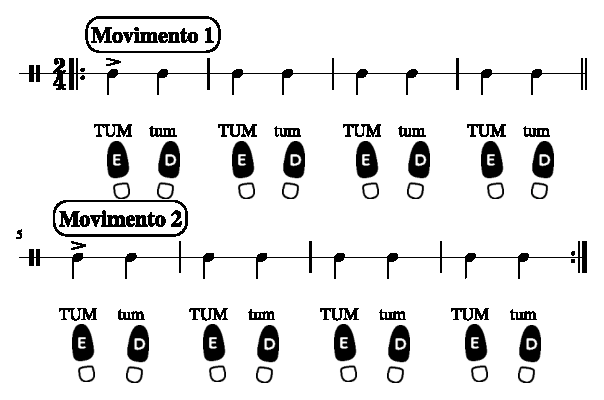
\includegraphics[width=0.99\textwidth]{chapters/cap-musicalidade/treino-fraseio0-1.eps}
    \caption{Duas frases coreográficas de 4 compassos.}
    \label{fig:frasecoreografica0}
\end{figure}

\begin{example}[Dançando em frases de 4 compassos:](2 movimentos)
De forma similar ao Exemplo \ref{ex:usandofrases1},
usaremos uma frase de 8 tempos, 
e usando uma distribuição de tempos dos movimentos, como na Figura \ref{fig:frasecoreografica1a}, 
podemos escolher distintos tipos de movimentos para as duas  frases coreográficas, 
como\footnote{Sim 
se quer agregar um pouco mais de complexidade ao exercício,
pode-se dar palmas no primeiro tempo de cada frase musical.}:
\begin{itemize}
\item \textbf{movimento 1:} realizar um balanço.
\item \textbf{movimento 2:} realizar o cruzado.
\end{itemize}
Outra  escolha alternativa de movimentos pode ser:
\begin{itemize}
\item \textbf{movimento 1:} realizar um balanço.
\item \textbf{movimento 2:} realizar o frente trás (básico linear).
\end{itemize}
Em ambos casos devemos seguir a distribuição de tempos indicada no último compasso de cada frase 
para ir ao movimento seguinte.
\end{example}

\begin{figure}[!h]
    \centering
    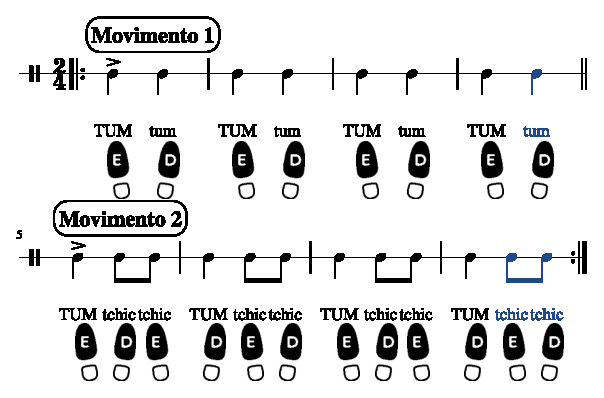
\includegraphics[width=0.99\textwidth]{chapters/cap-musicalidade/treino-fraseio1a-1.eps}
    \caption{Duas frases coreográficas de 4 compassos.}
    \label{fig:frasecoreografica1a}
\end{figure}


\begin{example}[Dançando em frases de 4 compassos:](3 movimentos)
Primeiro escolheremos uma música com frases de 4 compassos, 
como ``Disritmia'' interpretado por Martinho da Vila,
ou algumas das mostradas no Exemplo \ref{ex:frasesde4compassos}.
Logo procederemos a executar em cada frase musical uma frase coreográfica.
A primeira frase coreográfica leva o nome ``movimento 1'', 
a segunda ``movimento 2''  e a terceira ``movimento 3''.


Com a distribuição de tempos dos movimentos, da Figura \ref{fig:frasecoreografica2a}, 
podemos escolher distintos tipos de movimentos para as frases coreográficas, 
como\footnote{Sim 
se quer agregar um pouco mais de complexidade ao exercício,
pode-se dar palmas no primeiro tempo de cada frase musical.}:
\begin{itemize}
\item \textbf{movimento 1:} realizar um balanço.
\item \textbf{movimento 2:} realizar o cruzado.
\item \textbf{movimento 3:} realizar o frente trás (básico linear).
\end{itemize}
Em todos casos devemos seguir a distribuição de tempos indicada no ultimo compasso de cada frase para ir ao movimento seguinte.

\end{example}

\begin{figure}[!h]
    \centering
    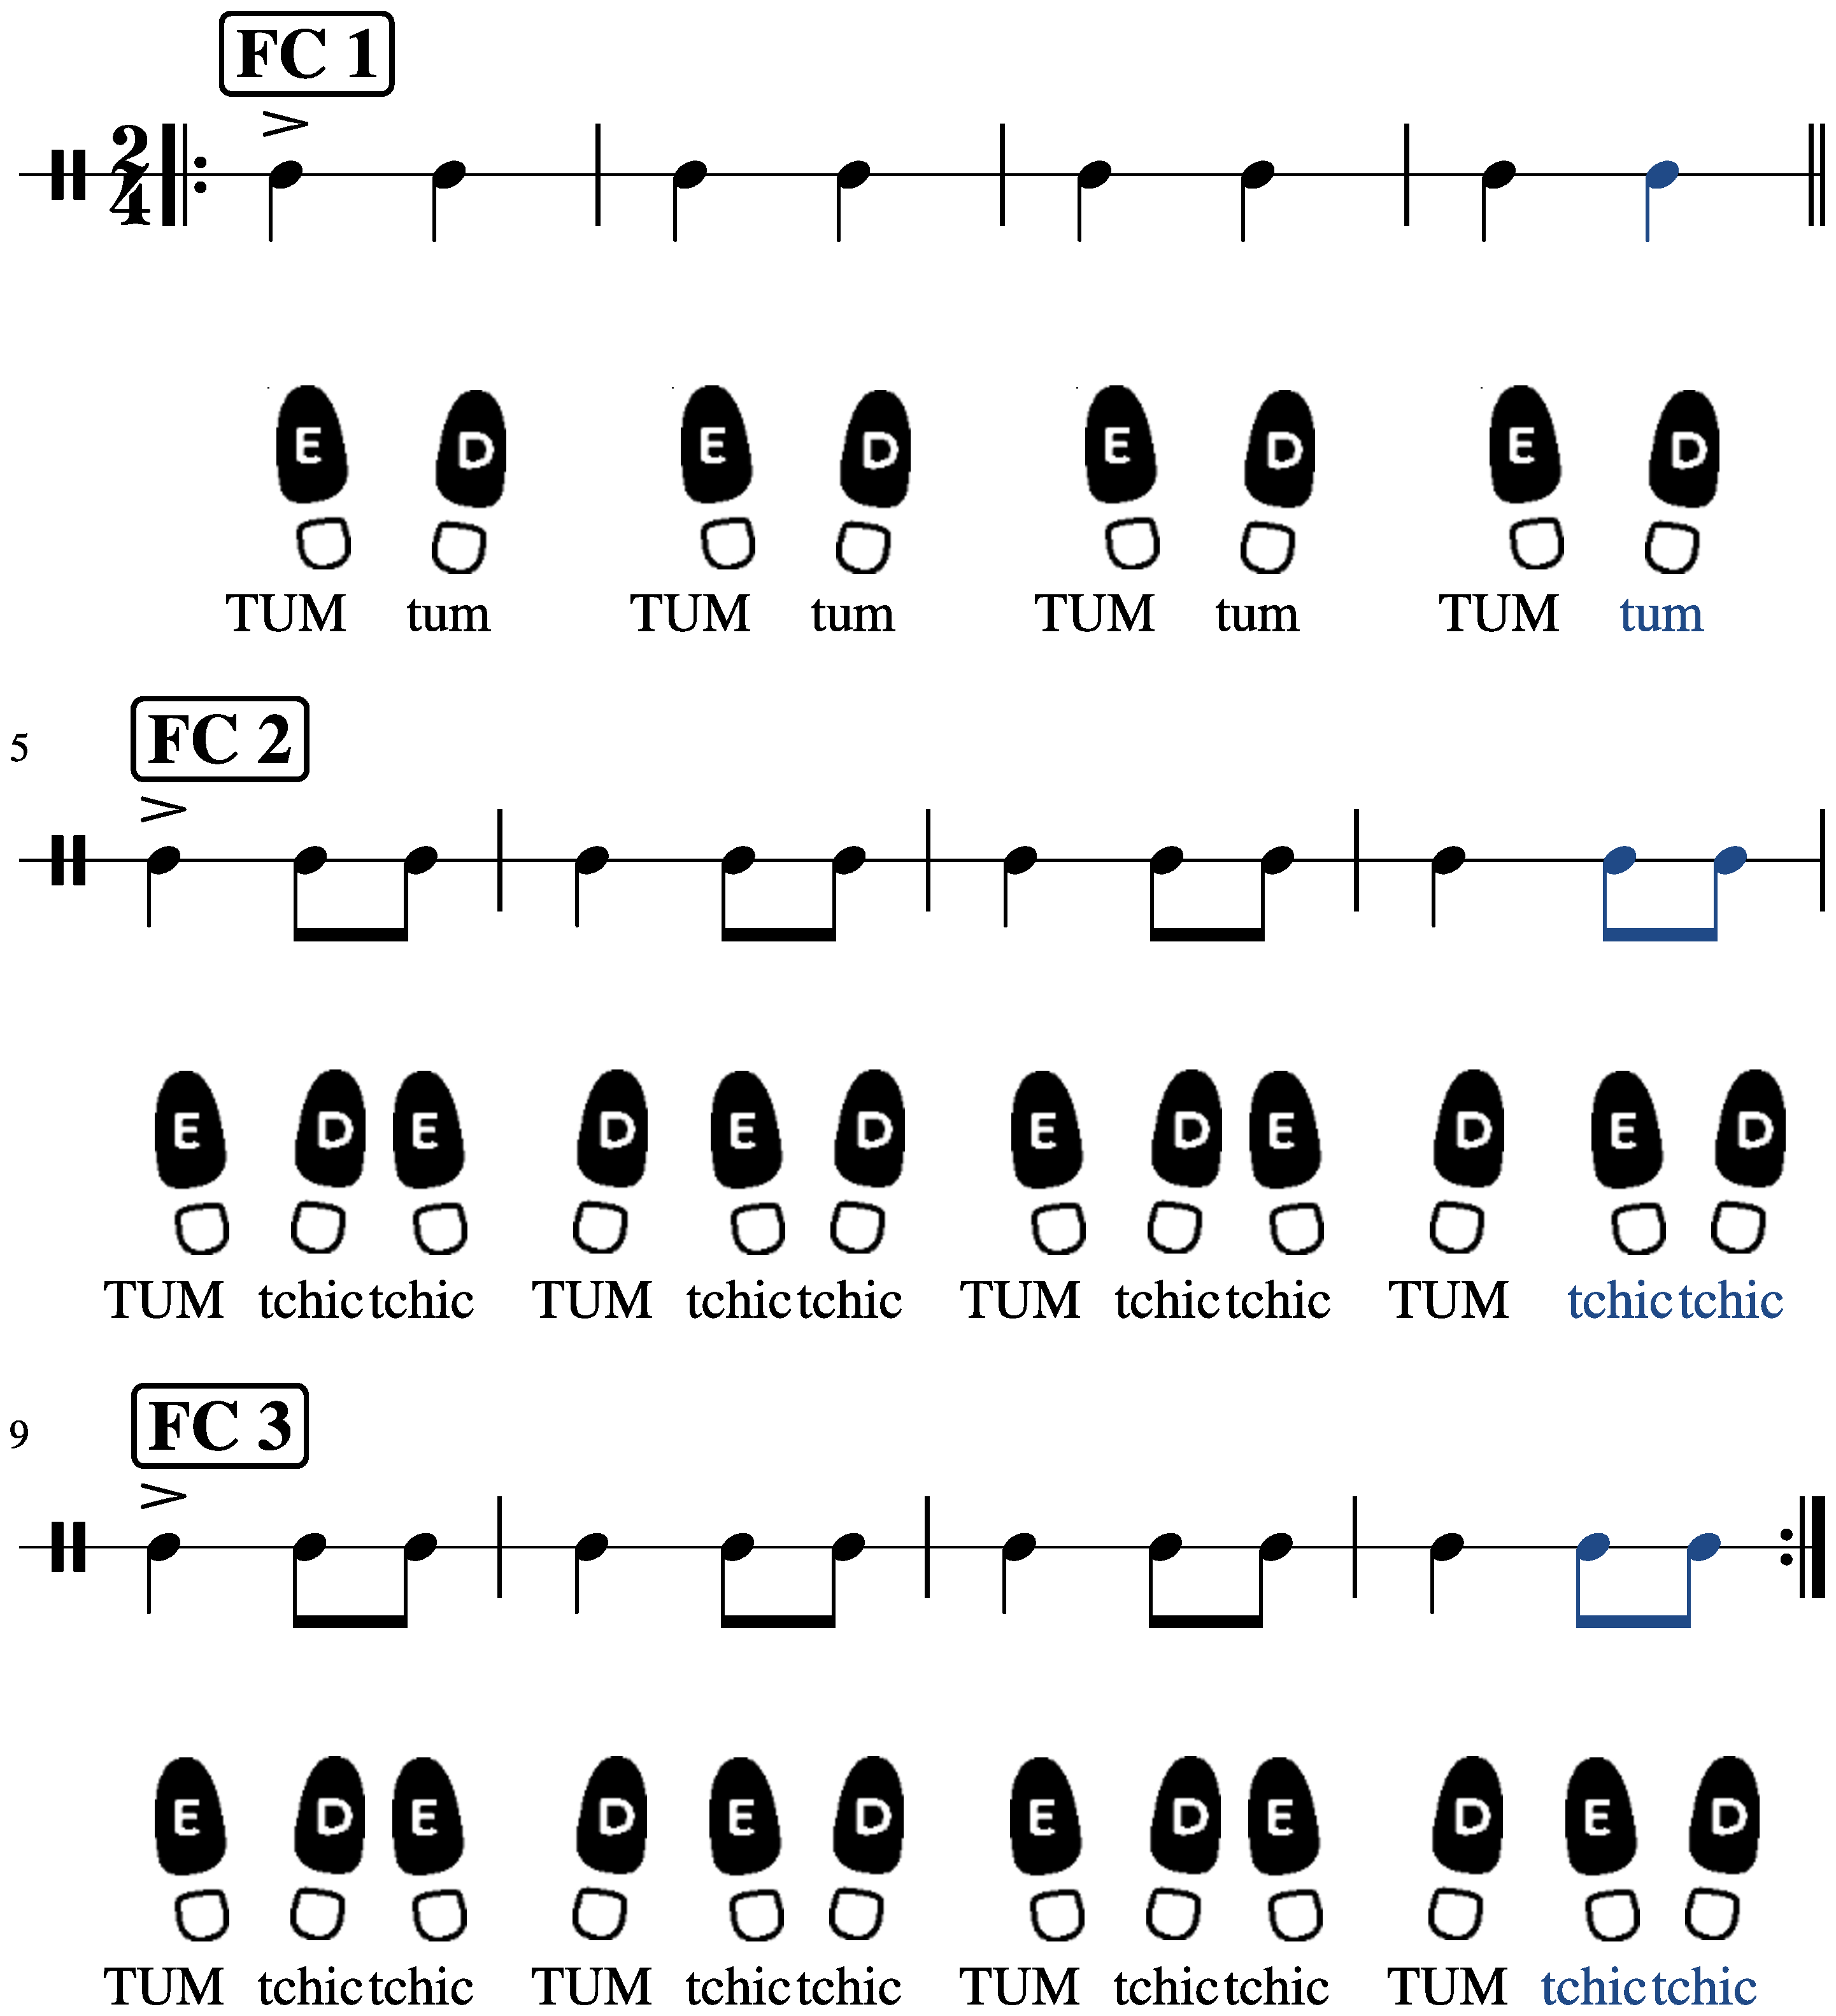
\includegraphics[width=0.9\textwidth]{chapters/cap-musicalidade/treino-fraseio2a-1.eps}
    \caption{Duas frases coreográficas de 4 compassos.}
    \label{fig:frasecoreografica2a}
\end{figure}

\begin{comment}
\subsection{Interpretando o tipo de final da frase}
\begin{itemize}
\item Si tentamos dançar no tempo forte, conhecer a existência de ambos tipos de final de frase, 
no ajuda a ter certeza que estamos indo bem com o tempo, e que não somos nos que erramos achando o tempo forte,
e sim, que existe mais de um tipo de final de frase, e que este foi diferente, foi suspensivo.
E não nos deixaremos enganar por finais suspensivos sincopados (que parecem conclusivos),
e estaremos mais seguros de nossa dança.
\item Uma vez temos ciência da existência de ambos tipos de final, 
podemos usar suas particularidades. Por exemplo,
uma frase com final conclusivo indica o fim, literal, de uma ideia musical, 
pelo que si desejamos ter coerência com a música, 
nosso movimento e parada deve demostrar a mesma resolução,
e dar a ideia de que o relato de nossa dança acabou de expressar uma ideia completa;
para isto podemos fazer um movimento explosivo com pausa abrupta, 
ou agregar uma postura final, ou tao simples como um abraço elegante com ponto final.
Por outro lado, se o final de frase musical é suspensivo, 
a ideia transmitida tem uma sensação de pergunta,
ou de uma resposta meditativa que se apaga aos poucos e pede uma reflexão ao ouvinte,
em outras palavras um assunto não completamente  concluído.
Nesse sentido, se nosso objetivo é ter uma coerência com a música,
o relato que expressa nossa dança deve dar essa sensação de uma ideia que se apaga aos poucos,
ou de pergunta; por exemplo, isto se consegue dando um passo final em tempo forte,
seguido de movimentos corporais no lugar até a ultima nota musical.
\end{itemize}
\end{comment}



